\PassOptionsToPackage{unicode=true}{hyperref} % options for packages loaded elsewhere
\PassOptionsToPackage{hyphens}{url}
%
\documentclass[ignorenonframetext,]{beamer}
\usepackage{pgfpages}
\setbeamertemplate{caption}[numbered]
\setbeamertemplate{caption label separator}{: }
\setbeamercolor{caption name}{fg=normal text.fg}
\beamertemplatenavigationsymbolsempty
% Prevent slide breaks in the middle of a paragraph:
\widowpenalties 1 10000
\raggedbottom
\setbeamertemplate{part page}{
\centering
\begin{beamercolorbox}[sep=16pt,center]{part title}
  \usebeamerfont{part title}\insertpart\par
\end{beamercolorbox}
}
\setbeamertemplate{section page}{
\centering
\begin{beamercolorbox}[sep=12pt,center]{part title}
  \usebeamerfont{section title}\insertsection\par
\end{beamercolorbox}
}
\setbeamertemplate{subsection page}{
\centering
\begin{beamercolorbox}[sep=8pt,center]{part title}
  \usebeamerfont{subsection title}\insertsubsection\par
\end{beamercolorbox}
}
\AtBeginPart{
  \frame{\partpage}
}
\AtBeginSection{
  \ifbibliography
  \else
    \frame{\sectionpage}
  \fi
}
\AtBeginSubsection{
  \frame{\subsectionpage}
}
\usepackage{lmodern}
\usepackage{amssymb,amsmath}
\usepackage{ifxetex,ifluatex}
\usepackage{fixltx2e} % provides \textsubscript
\ifnum 0\ifxetex 1\fi\ifluatex 1\fi=0 % if pdftex
  \usepackage[T1]{fontenc}
  \usepackage[utf8]{inputenc}
  \usepackage{textcomp} % provides euro and other symbols
\else % if luatex or xelatex
  \usepackage{unicode-math}
  \defaultfontfeatures{Ligatures=TeX,Scale=MatchLowercase}
\fi
% use upquote if available, for straight quotes in verbatim environments
\IfFileExists{upquote.sty}{\usepackage{upquote}}{}
% use microtype if available
\IfFileExists{microtype.sty}{%
\usepackage[]{microtype}
\UseMicrotypeSet[protrusion]{basicmath} % disable protrusion for tt fonts
}{}
\IfFileExists{parskip.sty}{%
\usepackage{parskip}
}{% else
\setlength{\parindent}{0pt}
\setlength{\parskip}{6pt plus 2pt minus 1pt}
}
\usepackage{hyperref}
\hypersetup{
            pdftitle={22100 - R for Bio Data Science},
            pdfauthor={Group 3: Laura Sans, Felix Pacheco, Jacob Kofoed, Begoña Bolos Sierra},
            pdfborder={0 0 0},
            breaklinks=true}
\urlstyle{same}  % don't use monospace font for urls
\newif\ifbibliography
\usepackage{graphicx,grffile}
\makeatletter
\def\maxwidth{\ifdim\Gin@nat@width>\linewidth\linewidth\else\Gin@nat@width\fi}
\def\maxheight{\ifdim\Gin@nat@height>\textheight\textheight\else\Gin@nat@height\fi}
\makeatother
% Scale images if necessary, so that they will not overflow the page
% margins by default, and it is still possible to overwrite the defaults
% using explicit options in \includegraphics[width, height, ...]{}
\setkeys{Gin}{width=\maxwidth,height=\maxheight,keepaspectratio}
\setlength{\emergencystretch}{3em}  % prevent overfull lines
\providecommand{\tightlist}{%
  \setlength{\itemsep}{0pt}\setlength{\parskip}{0pt}}
\setcounter{secnumdepth}{0}

% set default figure placement to htbp
\makeatletter
\def\fps@figure{htbp}
\makeatother


\title{22100 - R for Bio Data Science}
\providecommand{\subtitle}[1]{}
\subtitle{Spring 2020 - Group project}
\author{Group 3: Laura Sans, Felix Pacheco, Jacob Kofoed, Begoña Bolos Sierra}
\date{27-APR-2020}

\begin{document}
\frame{\titlepage}

\begin{frame}

\end{frame}

\begin{frame}{Project aims}
\protect\hypertarget{project-aims}{}

\begin{itemize}
\tightlist
\item
  Produce R script machine learning toolbox for protein and peptide
  bio-activities.
\item
  Features:

  \begin{itemize}
  \tightlist
  \item
    Support for both sequence or variant input.
  \item
    Support for several sequence encoders.
  \item
    Support for sequence based calculations.
  \item
    Support for several models.
  \item
    Visualization options.
  \end{itemize}
\end{itemize}

\end{frame}

\begin{frame}{R script overview 1}
\protect\hypertarget{r-script-overview-1}{}

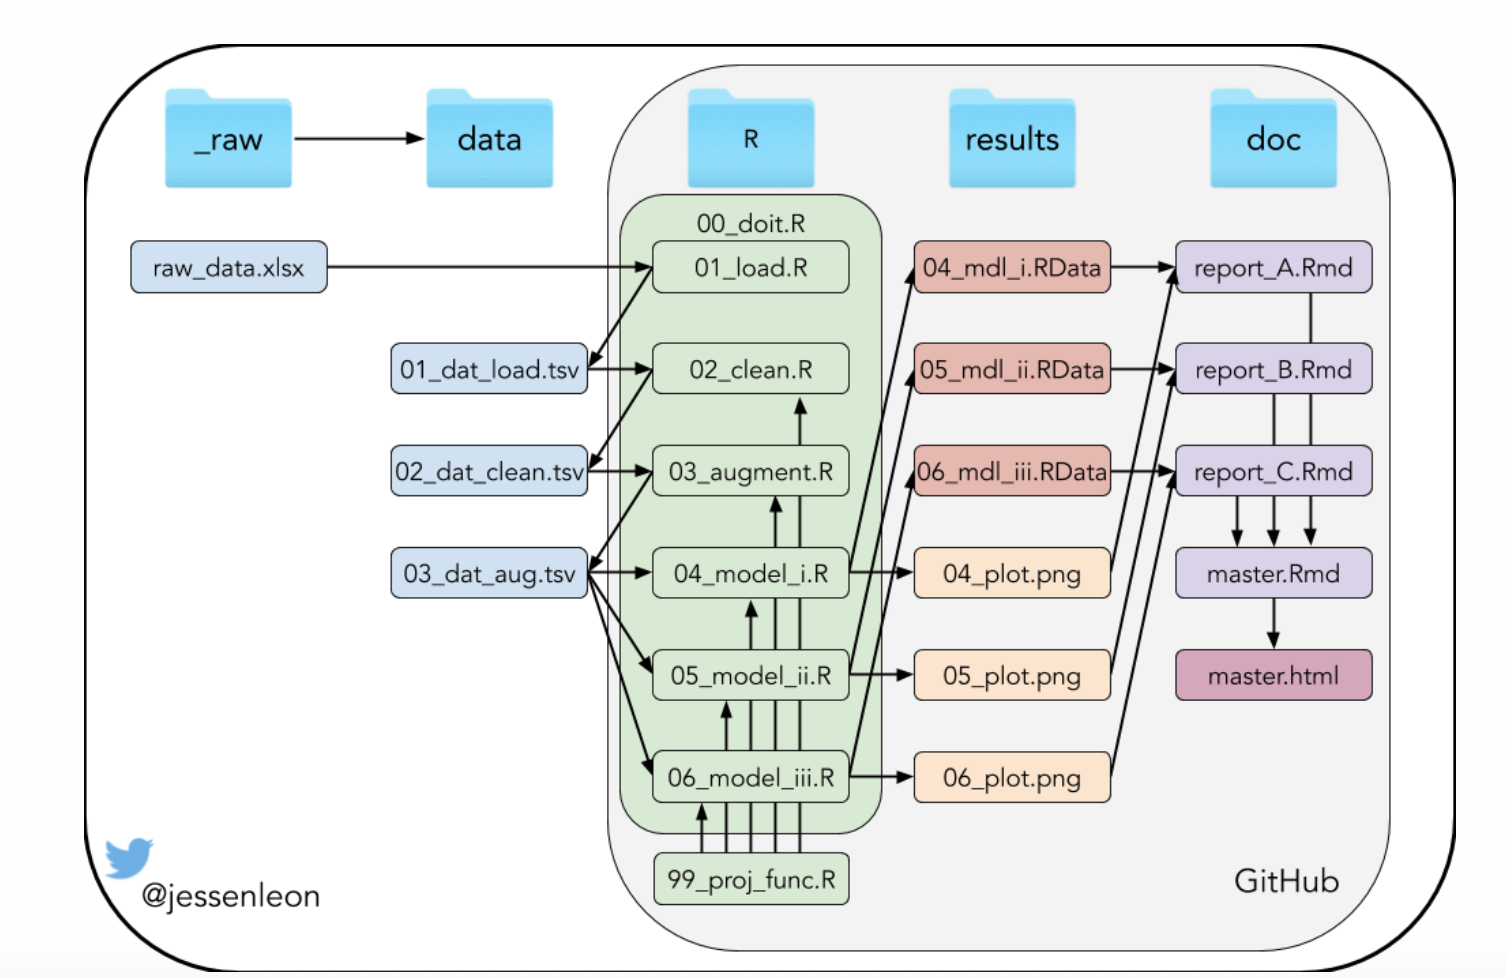
\includegraphics[width=5.20833in,height=\textheight]{project_organisation.png}

\begin{itemize}
\tightlist
\item
  00\_do\_it.R

  \begin{itemize}
  \tightlist
  \item
    Main program and loading of packages
  \end{itemize}
\item
  01\_load.R

  \begin{itemize}
  \tightlist
  \item
    Load: Encoding matrices, peptide and protein variant information and
    associated bio data
  \item
    Save: All loaded data in .tsv format
  \end{itemize}
\end{itemize}

\end{frame}

\begin{frame}{R script overview 2}
\protect\hypertarget{r-script-overview-2}{}

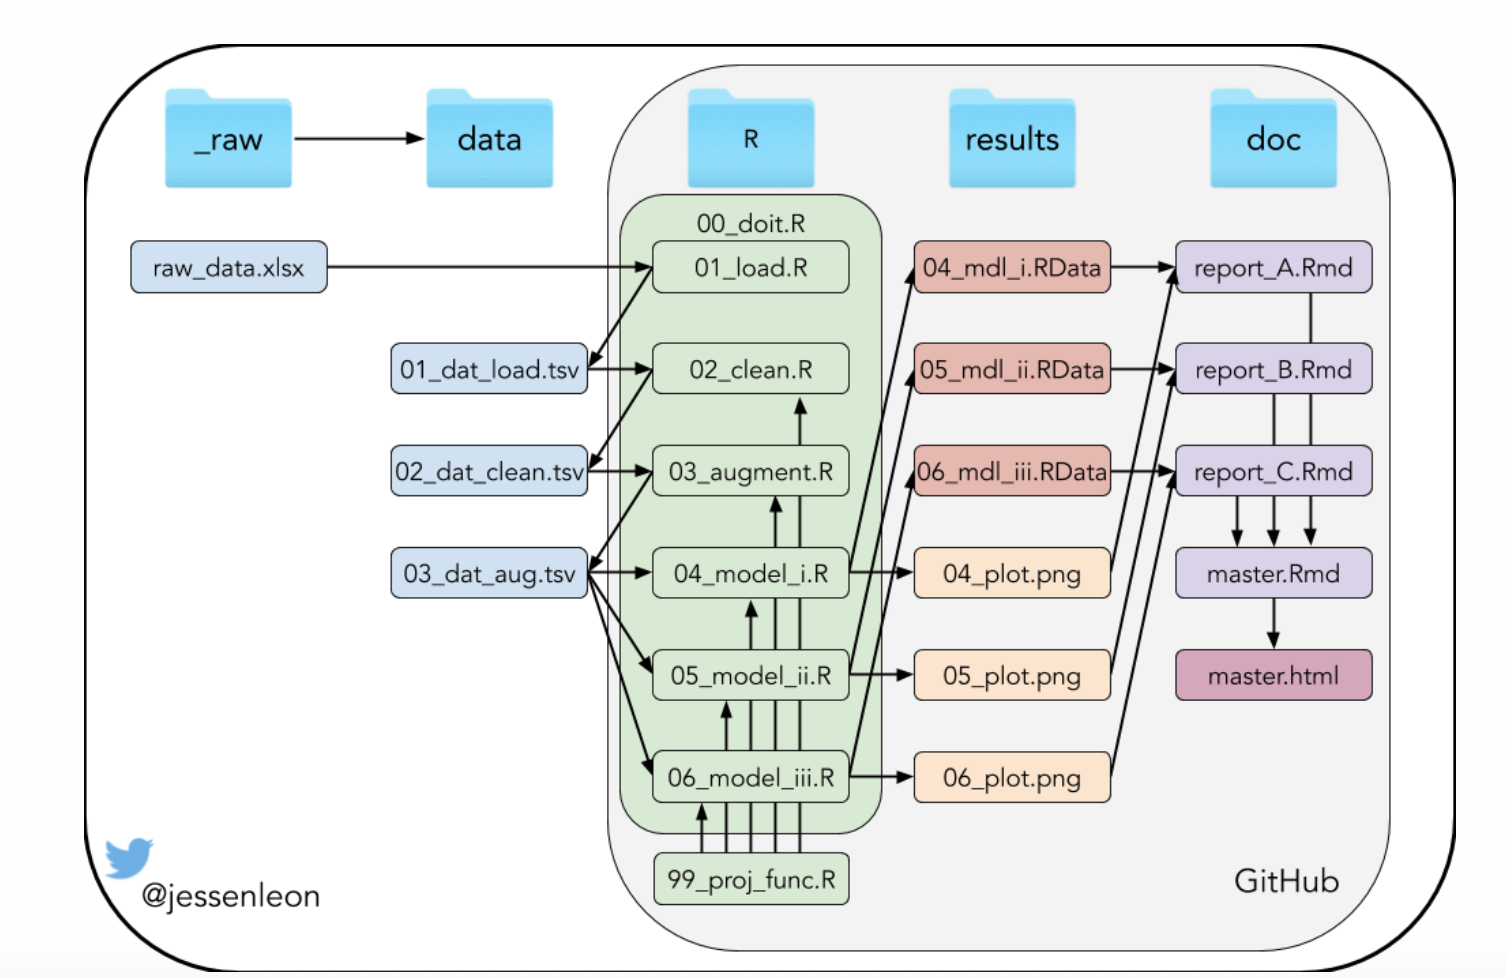
\includegraphics[width=5.20833in,height=\textheight]{project_organisation.png}

\begin{itemize}
\tightlist
\item
  02\_clean.R

  \begin{itemize}
  \tightlist
  \item
    Load: Load data from 01\_load.R
  \item
    Wrangle data: Remove NaN, fixes
  \item
    Save cleansed data in .tsv format
  \end{itemize}
\item
  03\_augment.R

  \begin{itemize}
  \tightlist
  \item
    Load data from 02\_clean.R
  \item
    Augment data: Calculate sequences, descriptors, properties
  \item
    Save augmente data in .tsv format
  \end{itemize}
\end{itemize}

\end{frame}

\begin{frame}{R script overview 3}
\protect\hypertarget{r-script-overview-3}{}

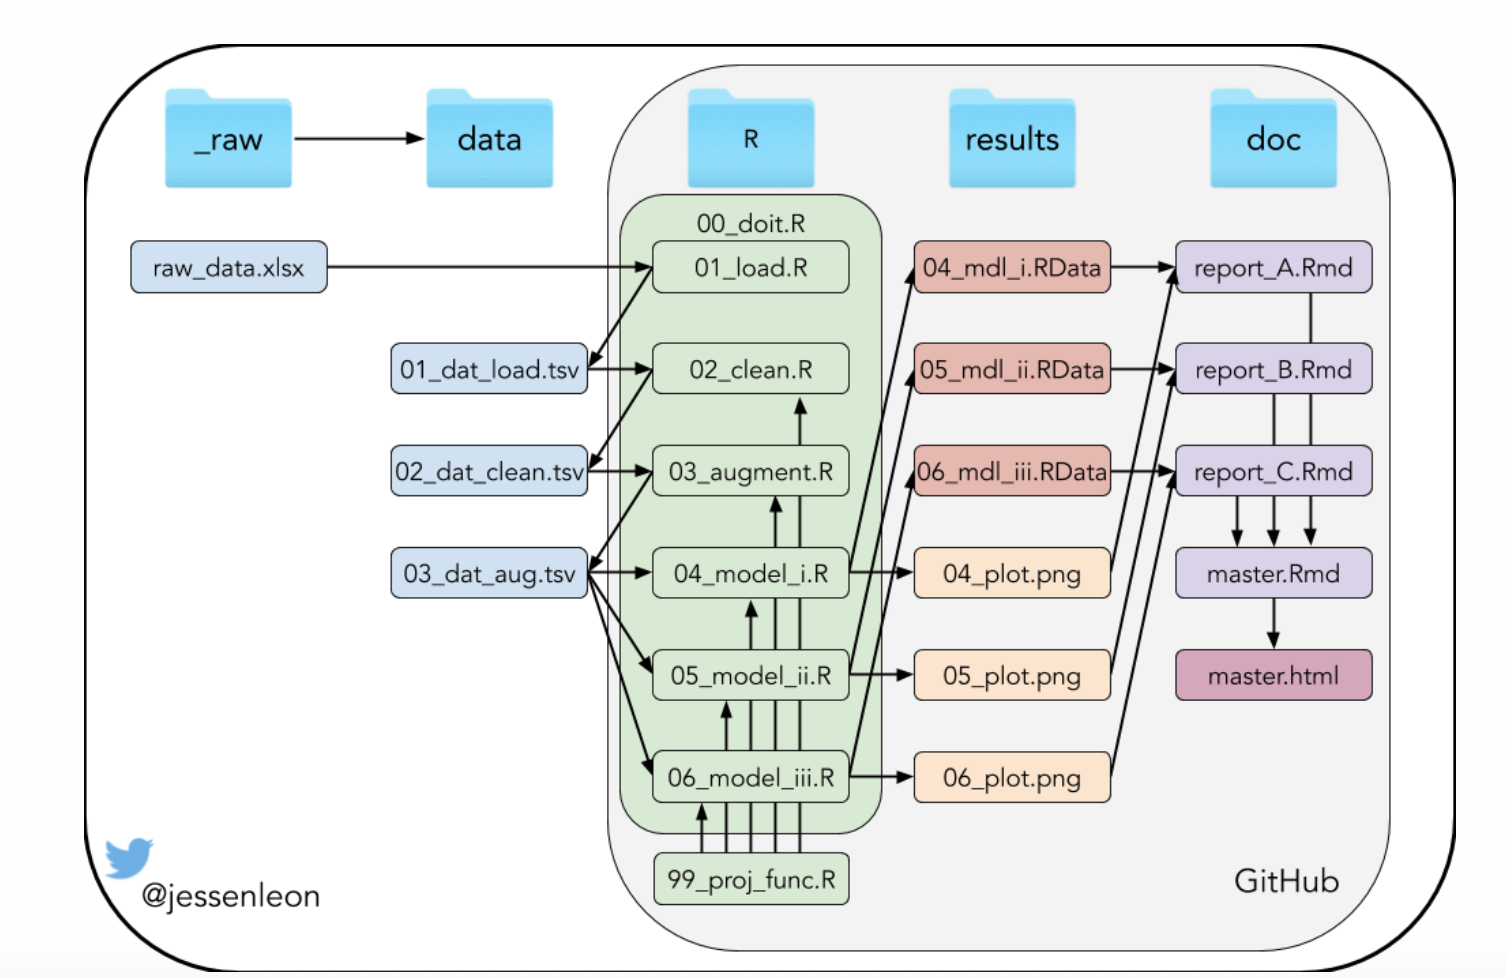
\includegraphics[width=5.20833in,height=\textheight]{project_organisation.png}

\begin{itemize}
\tightlist
\item
  04\_model\_i.R

  \begin{itemize}
  \tightlist
  \item
    Load augmented data
  \item
    Perform model fitting
  \item
    Predict unknowns
  \item
    Plotting and reporting
  \end{itemize}
\end{itemize}

\end{frame}

\begin{frame}{R script overview 4}
\protect\hypertarget{r-script-overview-4}{}

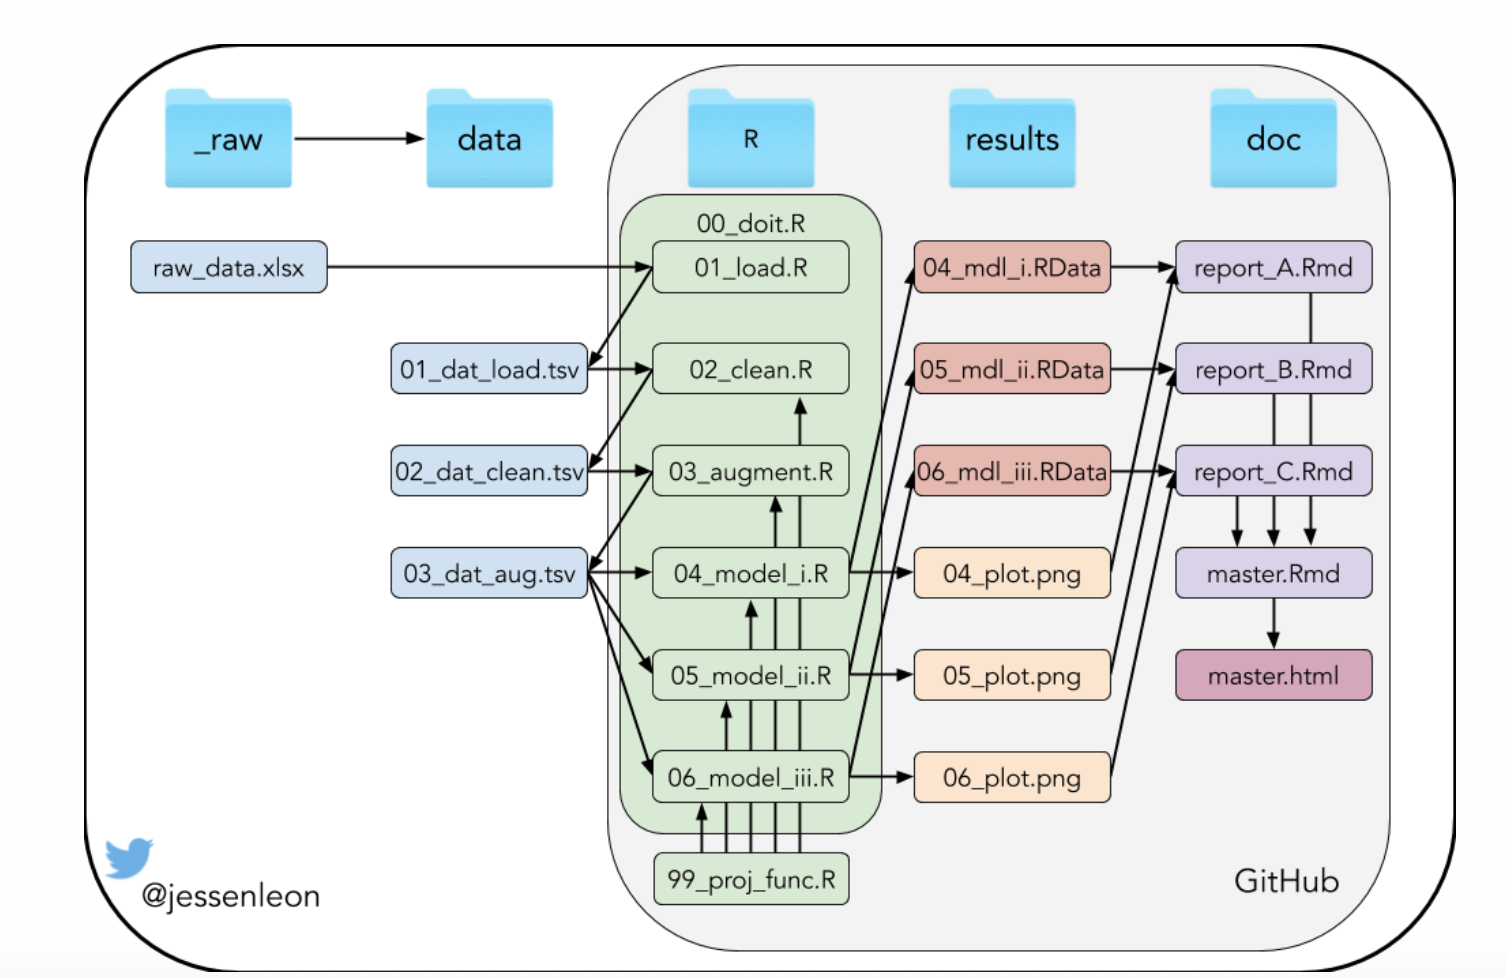
\includegraphics[width=5.20833in,height=\textheight]{project_organisation.png}

\begin{itemize}
\tightlist
\item
  99\_proj\_func.R

  \begin{itemize}
  \tightlist
  \item
    Sequence encoder
  \item
    Sequence generator
  \item
    \ldots{}
  \end{itemize}
\end{itemize}

\end{frame}

\begin{frame}{Data peptide and protein data sources}
\protect\hypertarget{data-peptide-and-protein-data-sources}{}

\begin{itemize}
\tightlist
\item
  Ideas for sequence / variant effects:

  \begin{itemize}
  \tightlist
  \item
    \url{https://www.mavedb.org/} is a public repository for datasets
    from Multiplexed Assays of Variant Effect (MAVEs), such as those
    generated by deep mutational scanning (DMS) or massively parallel
    reporter assay (MPRA) experiments. RESTful API.
  \item
    Other scientific litterature\ldots{}
  \end{itemize}
\item
  Ideas for sequence encoding matrices

  \begin{itemize}
  \tightlist
  \item
    BLOSUM - Physicochemical and substitution matrix
  \item
    Z-scales - Physicochemical
  \item
    T-scales - Topological
  \item
    MSWHIM - 3D electrostatic potential
  \end{itemize}
\end{itemize}

\end{frame}

\begin{frame}{Machine learning toolbox}
\protect\hypertarget{machine-learning-toolbox}{}

\begin{itemize}
\item
  Ideas for supported machine learning framework:

  \begin{itemize}
  \tightlist
  \item
    Gaussian Process Regression.
  \item
    Artificial Neutral Network.
  \item
    ElasticNet Regression.
  \end{itemize}
\end{itemize}

\end{frame}

\begin{frame}{Distribution of tasks, week 18}
\protect\hypertarget{distribution-of-tasks-week-18}{}

\begin{itemize}
\item
  Laura: Descriptors and function for translating
\item
  Jacob: Sequence generation
\item
  Felix, Begoña: Machine learning tool boox
\item
  Project state EOW - functional preprocessing, first steps with machine
  learning toolbox
\end{itemize}

\end{frame}

\begin{frame}{Distribution of tasks, week 19}
\protect\hypertarget{distribution-of-tasks-week-19}{}

\end{frame}

\end{document}
